% ---------------------------------------------------------------------------
% fig_workflow_compare.tex
%
% Comparison of the symbol-alignment development workflow: the traditional
% manual procedure versus A2L-RAGAlign (ours).  Included from main.tex:
%
%     % ---------------------------------------------------------------------------
% fig_workflow_compare.tex
%
% Comparison of the symbol-alignment development workflow: the traditional
% manual procedure versus A2L-RAGAlign (ours).  Included from main.tex:
%
%     % ---------------------------------------------------------------------------
% fig_workflow_compare.tex
%
% Comparison of the symbol-alignment development workflow: the traditional
% manual procedure versus A2L-RAGAlign (ours).  Included from main.tex:
%
%     % ---------------------------------------------------------------------------
% fig_workflow_compare.tex
%
% Comparison of the symbol-alignment development workflow: the traditional
% manual procedure versus A2L-RAGAlign (ours).  Included from main.tex:
%
%     \input{figures/fig_workflow_compare}
%
% ASCII-only on purpose: the paper is built with pdfLaTeX (no CJK support).
%
% Structure: three phase groups (candidate & evidence / validation & decision
% / traceability & review) over six stage columns, one row per workflow.
% Every cell follows the same three-line schema
%
%     <action> / <mechanism> / <outcome property>
%
% so that the two rows are directly comparable column by column, and the
% difference between them reads as "who executes which stage, with what
% machinery, and what is recorded".  All icons are drawn with plain TikZ
% paths: the figure needs no external image files and stays pure vector in
% the typeset PDF.
%
% Cell lines are kept at or below 14 characters so that no cell wraps and
% both rows keep one common baseline grid.
% ---------------------------------------------------------------------------
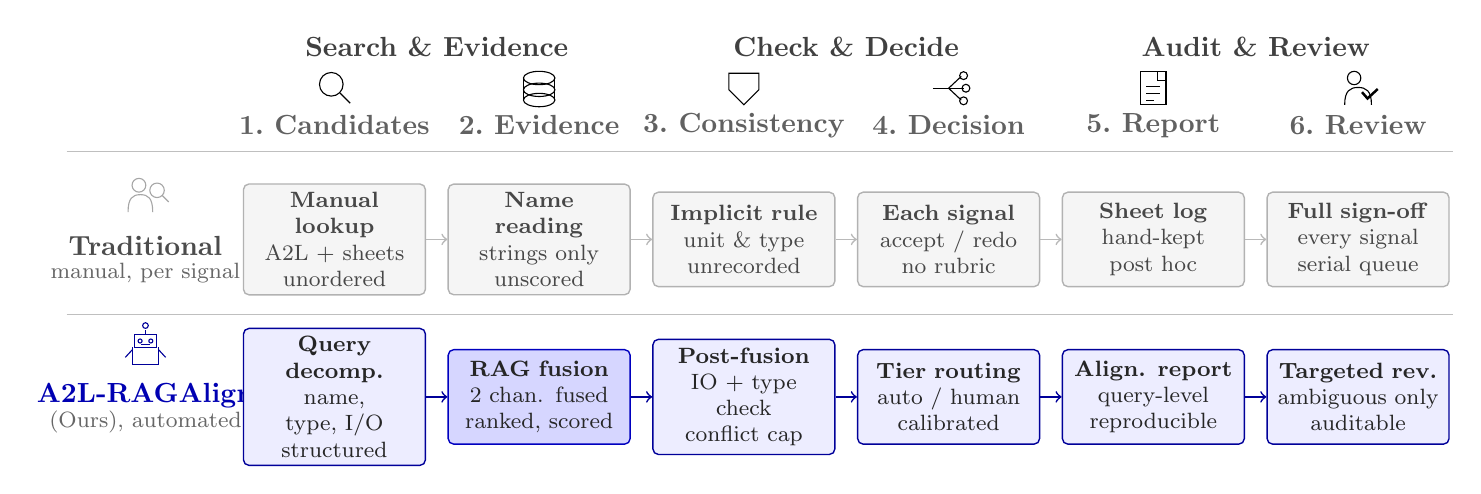
\begin{tikzpicture}[
    font=\footnotesize,
    every node/.style={align=center},
    colhead/.style={font=\bfseries, text=black!62},
    grouplbl/.style={font=\bfseries, text=black!75, fill=white,
                     inner xsep=4pt},
    rowname/.style={font=\bfseries},
    rowsub/.style={text=black!60},
    cell/.style={font=\footnotesize, text width=2.10cm, inner sep=3pt,
               minimum height=1.20cm, line width=0.5pt, rounded corners=2pt},
    man/.style={cell, draw=gray!60, fill=gray!8, text=black!72},
    rag/.style={cell, draw=blue!60!black, fill=blue!7, text=black!85},
    core/.style={rag, draw=blue!75!black, fill=blue!16},
    flowm/.style={->, line width=0.6pt, draw=gray!55},
    flowr/.style={->, line width=0.6pt, draw=blue!60!black},
    rule/.style={line width=0.4pt, draw=black!25},
    grouprule/.style={line width=0.5pt, draw=black!45},
    % ---- stage icons (line art, origin = icon centre) --------------------
    pics/search/.style={code={
        \draw (-0.04,0.05) circle (0.15);
        \draw (0.07,-0.06) -- (0.20,-0.19);}},
    pics/database/.style={code={
        \draw (0,0.13) ellipse (0.20 and 0.085);
        \draw (-0.20,0.13) -- (-0.20,-0.14);
        \draw (0.20,0.13) -- (0.20,-0.14);
        \draw (0,-0.02) ellipse (0.20 and 0.085);
        \draw (0,-0.15) ellipse (0.20 and 0.085);}},
    pics/shield/.style={code={
        \draw (-0.19,0.19) -- (0.19,0.19) -- (0.19,-0.02)
              -- (0,-0.21) -- (-0.19,-0.02) -- cycle;}},
    pics/route/.style={code={
        \draw (-0.20,0.0) -- (0.0,0.0);
        \draw (0.0,0.0) -- (0.16,0.15);
        \draw (0.0,0.0) -- (0.20,0.0);
        \draw (0.0,0.0) -- (0.16,-0.15);
        \draw (0.19,0.16) circle (0.05);
        \draw (0.22,0.0) circle (0.05);
        \draw (0.19,-0.16) circle (0.05);}},
    pics/report/.style={code={
        \draw (-0.16,-0.21) rectangle (0.16,0.21);
        \draw (0.05,0.21) -- (0.05,0.10) -- (0.16,0.10);
        \draw (-0.09,0.02) -- (0.09,0.02);
        \draw (-0.09,-0.07) -- (0.09,-0.07);
        \draw (-0.09,-0.16) -- (0.01,-0.16);}},
    pics/expert/.style={code={
        \draw (-0.05,0.13) circle (0.085);
        \draw (-0.17,-0.21) .. controls (-0.17,-0.03) and (-0.10,0.01)
              .. (0.0,0.01) .. controls (0.10,0.01) and (0.17,-0.03)
              .. (0.17,-0.21);
        \draw[line width=0.9pt] (0.05,-0.05) -- (0.12,-0.13) -- (0.25,-0.01);}},
    pics/person/.style={code={
        \begin{scope}[scale=0.92]
            \draw (-0.09,0.15) circle (0.095);
            \draw (-0.24,-0.22) .. controls (-0.24,-0.03) and (-0.18,0.02) .. (-0.07,0.02)
                  .. controls (0.04,0.02) and (0.10,-0.03) .. (0.10,-0.22);
            \draw (0.16,0.08) circle (0.10);
            \draw (0.23,0.01) -- (0.32,-0.08);
        \end{scope}}},
    pics/robot/.style={code={
        % yshift aligns the visual centre of the robot with the
        % visual centre of the person icon in the row above
        \begin{scope}[scale=0.80, yshift=-0.065cm]
            \draw (0,0.24) -- (0,0.32);
            \draw (0,0.385) circle (0.045);
            \draw (-0.17,0.24) rectangle (0.17,0.04);
            \draw (-0.085,0.14) circle (0.032);
            \draw (0.085,0.14) circle (0.032);
            \draw (-0.07,0.08) -- (0.07,0.08);
            \draw (-0.21,0.04) -- (-0.21,-0.24) -- (0.21,-0.24) -- (0.21,0.04);
            \draw (-0.21,0.0) -- (-0.32,-0.12);
            \draw (0.21,0.0) -- (0.32,-0.12);
        \end{scope}}},
]
% ---------------------------- phase groups ---------------------------------
\draw[grouprule] (3.6,3.45) -- (6.2,3.45);
\draw[grouprule] (3.6,3.45) -- (3.6,3.28);
\draw[grouprule] (6.2,3.45) -- (6.2,3.28);
\node[grouplbl] at (4.9,3.45) {Search \& Evidence};

\draw[grouprule] (8.8,3.45) -- (11.4,3.45);
\draw[grouprule] (8.8,3.45) -- (8.8,3.28);
\draw[grouprule] (11.4,3.45) -- (11.4,3.28);
\node[grouplbl] at (10.1,3.45) {Check \& Decide};

\draw[grouprule] (14.0,3.45) -- (16.6,3.45);
\draw[grouprule] (14.0,3.45) -- (14.0,3.28);
\draw[grouprule] (16.6,3.45) -- (16.6,3.28);
\node[grouplbl] at (15.3,3.45) {Audit \& Review};
% ---------------------------- column headers ------------------------------
\foreach \x/\ic/\t in {3.6/search/{1.\ Candidates},
                       6.2/database/{2.\ Evidence},
                       8.8/shield/{3.\ Consistency},
                       11.4/route/{4.\ Decision},
                       14.0/report/{5.\ Report},
                       16.6/expert/{6.\ Review}} {
    \pic at (\x,2.92) {\ic};
    \node[colhead] at (\x,2.45) {\t};
}
\draw[rule] (0.2,2.12) -- (17.8,2.12);
% ======================= row A: traditional workflow ======================
\begin{scope}[draw=gray!70]
    \pic at (1.2,1.55) {person};
\end{scope}
\node[rowname, text=black!70] at (1.2,0.92) {Traditional};
\node[rowsub] at (1.2,0.58) {manual, per signal};
\node[man] (a1) at (3.6,1.0)
    {\textbf{Manual lookup}\\A2L + sheets\\unordered};
\node[man] (a2) at (6.2,1.0)
    {\textbf{Name reading}\\strings only\\unscored};
\node[man] (a3) at (8.8,1.0)
    {\textbf{Implicit rule}\\unit \& type\\unrecorded};
\node[man] (a4) at (11.4,1.0)
    {\textbf{Each signal}\\accept / redo\\no rubric};
\node[man] (a5) at (14.0,1.0)
    {\textbf{Sheet log}\\hand-kept\\post hoc};
\node[man] (a6) at (16.6,1.0)
    {\textbf{Full sign-off}\\every signal\\serial queue};
\draw[flowm] (a1) -- (a2);
\draw[flowm] (a2) -- (a3);
\draw[flowm] (a3) -- (a4);
\draw[flowm] (a4) -- (a5);
\draw[flowm] (a5) -- (a6);
\draw[rule] (0.2,0.05) -- (17.8,0.05);
% ===================== row B: A2L-RAGAlign (ours) ========================
\begin{scope}[draw=blue!60!black]
    \pic at (1.2,-0.35) {robot};
\end{scope}
\node[rowname, text=blue!70!black] at (1.2,-0.98) {A2L-RAGAlign};
\node[rowsub] at (1.2,-1.32) {(Ours), automated};
\node[rag] (b1) at (3.6,-1.0)
    {\textbf{Query decomp.}\\name, type, I/O\\structured};
\node[core] (b2) at (6.2,-1.0)
    {\textbf{RAG fusion}\\2 chan. fused\\ranked, scored};
\node[rag] (b3) at (8.8,-1.0)
    {\textbf{Post-fusion}\\IO + type check\\conflict cap};
\node[rag] (b4) at (11.4,-1.0)
    {\textbf{Tier routing}\\auto / human\\calibrated};
\node[rag] (b5) at (14.0,-1.0)
    {\textbf{Align. report}\\query-level\\reproducible};
\node[rag] (b6) at (16.6,-1.0)
    {\textbf{Targeted rev.}\\ambiguous only\\auditable};
\draw[flowr] (b1) -- (b2);
\draw[flowr] (b2) -- (b3);
\draw[flowr] (b3) -- (b4);
\draw[flowr] (b4) -- (b5);
\draw[flowr] (b5) -- (b6);
\end{tikzpicture}

%
% ASCII-only on purpose: the paper is built with pdfLaTeX (no CJK support).
%
% Structure: three phase groups (candidate & evidence / validation & decision
% / traceability & review) over six stage columns, one row per workflow.
% Every cell follows the same three-line schema
%
%     <action> / <mechanism> / <outcome property>
%
% so that the two rows are directly comparable column by column, and the
% difference between them reads as "who executes which stage, with what
% machinery, and what is recorded".  All icons are drawn with plain TikZ
% paths: the figure needs no external image files and stays pure vector in
% the typeset PDF.
%
% Cell lines are kept at or below 14 characters so that no cell wraps and
% both rows keep one common baseline grid.
% ---------------------------------------------------------------------------
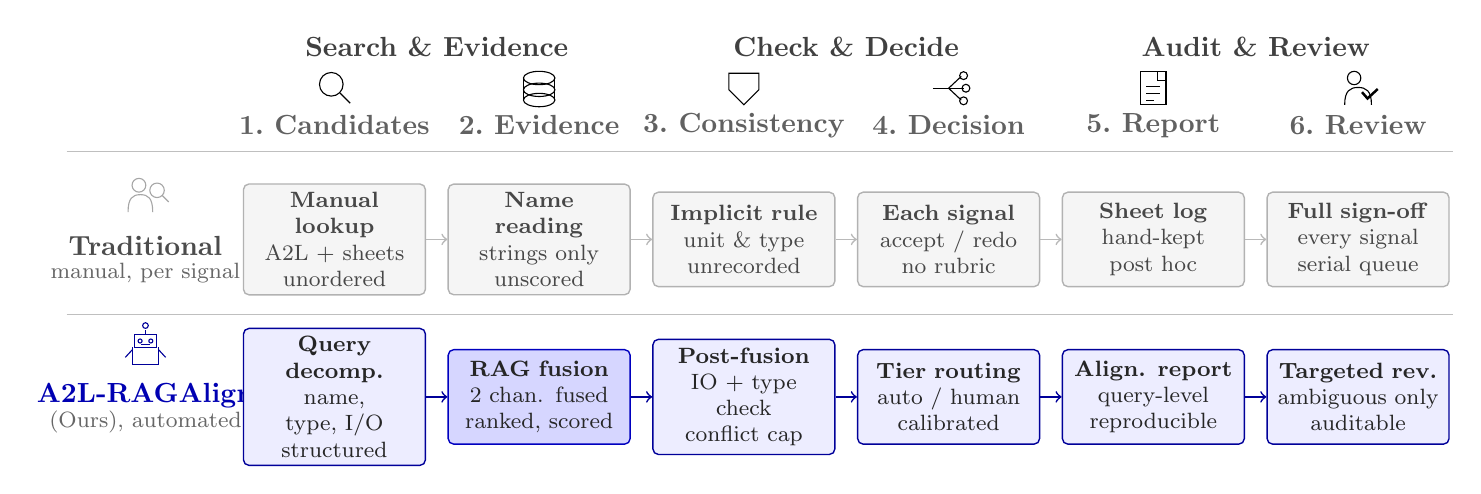
\begin{tikzpicture}[
    font=\footnotesize,
    every node/.style={align=center},
    colhead/.style={font=\bfseries, text=black!62},
    grouplbl/.style={font=\bfseries, text=black!75, fill=white,
                     inner xsep=4pt},
    rowname/.style={font=\bfseries},
    rowsub/.style={text=black!60},
    cell/.style={font=\footnotesize, text width=2.10cm, inner sep=3pt,
               minimum height=1.20cm, line width=0.5pt, rounded corners=2pt},
    man/.style={cell, draw=gray!60, fill=gray!8, text=black!72},
    rag/.style={cell, draw=blue!60!black, fill=blue!7, text=black!85},
    core/.style={rag, draw=blue!75!black, fill=blue!16},
    flowm/.style={->, line width=0.6pt, draw=gray!55},
    flowr/.style={->, line width=0.6pt, draw=blue!60!black},
    rule/.style={line width=0.4pt, draw=black!25},
    grouprule/.style={line width=0.5pt, draw=black!45},
    % ---- stage icons (line art, origin = icon centre) --------------------
    pics/search/.style={code={
        \draw (-0.04,0.05) circle (0.15);
        \draw (0.07,-0.06) -- (0.20,-0.19);}},
    pics/database/.style={code={
        \draw (0,0.13) ellipse (0.20 and 0.085);
        \draw (-0.20,0.13) -- (-0.20,-0.14);
        \draw (0.20,0.13) -- (0.20,-0.14);
        \draw (0,-0.02) ellipse (0.20 and 0.085);
        \draw (0,-0.15) ellipse (0.20 and 0.085);}},
    pics/shield/.style={code={
        \draw (-0.19,0.19) -- (0.19,0.19) -- (0.19,-0.02)
              -- (0,-0.21) -- (-0.19,-0.02) -- cycle;}},
    pics/route/.style={code={
        \draw (-0.20,0.0) -- (0.0,0.0);
        \draw (0.0,0.0) -- (0.16,0.15);
        \draw (0.0,0.0) -- (0.20,0.0);
        \draw (0.0,0.0) -- (0.16,-0.15);
        \draw (0.19,0.16) circle (0.05);
        \draw (0.22,0.0) circle (0.05);
        \draw (0.19,-0.16) circle (0.05);}},
    pics/report/.style={code={
        \draw (-0.16,-0.21) rectangle (0.16,0.21);
        \draw (0.05,0.21) -- (0.05,0.10) -- (0.16,0.10);
        \draw (-0.09,0.02) -- (0.09,0.02);
        \draw (-0.09,-0.07) -- (0.09,-0.07);
        \draw (-0.09,-0.16) -- (0.01,-0.16);}},
    pics/expert/.style={code={
        \draw (-0.05,0.13) circle (0.085);
        \draw (-0.17,-0.21) .. controls (-0.17,-0.03) and (-0.10,0.01)
              .. (0.0,0.01) .. controls (0.10,0.01) and (0.17,-0.03)
              .. (0.17,-0.21);
        \draw[line width=0.9pt] (0.05,-0.05) -- (0.12,-0.13) -- (0.25,-0.01);}},
    pics/person/.style={code={
        \begin{scope}[scale=0.92]
            \draw (-0.09,0.15) circle (0.095);
            \draw (-0.24,-0.22) .. controls (-0.24,-0.03) and (-0.18,0.02) .. (-0.07,0.02)
                  .. controls (0.04,0.02) and (0.10,-0.03) .. (0.10,-0.22);
            \draw (0.16,0.08) circle (0.10);
            \draw (0.23,0.01) -- (0.32,-0.08);
        \end{scope}}},
    pics/robot/.style={code={
        % yshift aligns the visual centre of the robot with the
        % visual centre of the person icon in the row above
        \begin{scope}[scale=0.80, yshift=-0.065cm]
            \draw (0,0.24) -- (0,0.32);
            \draw (0,0.385) circle (0.045);
            \draw (-0.17,0.24) rectangle (0.17,0.04);
            \draw (-0.085,0.14) circle (0.032);
            \draw (0.085,0.14) circle (0.032);
            \draw (-0.07,0.08) -- (0.07,0.08);
            \draw (-0.21,0.04) -- (-0.21,-0.24) -- (0.21,-0.24) -- (0.21,0.04);
            \draw (-0.21,0.0) -- (-0.32,-0.12);
            \draw (0.21,0.0) -- (0.32,-0.12);
        \end{scope}}},
]
% ---------------------------- phase groups ---------------------------------
\draw[grouprule] (3.6,3.45) -- (6.2,3.45);
\draw[grouprule] (3.6,3.45) -- (3.6,3.28);
\draw[grouprule] (6.2,3.45) -- (6.2,3.28);
\node[grouplbl] at (4.9,3.45) {Search \& Evidence};

\draw[grouprule] (8.8,3.45) -- (11.4,3.45);
\draw[grouprule] (8.8,3.45) -- (8.8,3.28);
\draw[grouprule] (11.4,3.45) -- (11.4,3.28);
\node[grouplbl] at (10.1,3.45) {Check \& Decide};

\draw[grouprule] (14.0,3.45) -- (16.6,3.45);
\draw[grouprule] (14.0,3.45) -- (14.0,3.28);
\draw[grouprule] (16.6,3.45) -- (16.6,3.28);
\node[grouplbl] at (15.3,3.45) {Audit \& Review};
% ---------------------------- column headers ------------------------------
\foreach \x/\ic/\t in {3.6/search/{1.\ Candidates},
                       6.2/database/{2.\ Evidence},
                       8.8/shield/{3.\ Consistency},
                       11.4/route/{4.\ Decision},
                       14.0/report/{5.\ Report},
                       16.6/expert/{6.\ Review}} {
    \pic at (\x,2.92) {\ic};
    \node[colhead] at (\x,2.45) {\t};
}
\draw[rule] (0.2,2.12) -- (17.8,2.12);
% ======================= row A: traditional workflow ======================
\begin{scope}[draw=gray!70]
    \pic at (1.2,1.55) {person};
\end{scope}
\node[rowname, text=black!70] at (1.2,0.92) {Traditional};
\node[rowsub] at (1.2,0.58) {manual, per signal};
\node[man] (a1) at (3.6,1.0)
    {\textbf{Manual lookup}\\A2L + sheets\\unordered};
\node[man] (a2) at (6.2,1.0)
    {\textbf{Name reading}\\strings only\\unscored};
\node[man] (a3) at (8.8,1.0)
    {\textbf{Implicit rule}\\unit \& type\\unrecorded};
\node[man] (a4) at (11.4,1.0)
    {\textbf{Each signal}\\accept / redo\\no rubric};
\node[man] (a5) at (14.0,1.0)
    {\textbf{Sheet log}\\hand-kept\\post hoc};
\node[man] (a6) at (16.6,1.0)
    {\textbf{Full sign-off}\\every signal\\serial queue};
\draw[flowm] (a1) -- (a2);
\draw[flowm] (a2) -- (a3);
\draw[flowm] (a3) -- (a4);
\draw[flowm] (a4) -- (a5);
\draw[flowm] (a5) -- (a6);
\draw[rule] (0.2,0.05) -- (17.8,0.05);
% ===================== row B: A2L-RAGAlign (ours) ========================
\begin{scope}[draw=blue!60!black]
    \pic at (1.2,-0.35) {robot};
\end{scope}
\node[rowname, text=blue!70!black] at (1.2,-0.98) {A2L-RAGAlign};
\node[rowsub] at (1.2,-1.32) {(Ours), automated};
\node[rag] (b1) at (3.6,-1.0)
    {\textbf{Query decomp.}\\name, type, I/O\\structured};
\node[core] (b2) at (6.2,-1.0)
    {\textbf{RAG fusion}\\2 chan. fused\\ranked, scored};
\node[rag] (b3) at (8.8,-1.0)
    {\textbf{Post-fusion}\\IO + type check\\conflict cap};
\node[rag] (b4) at (11.4,-1.0)
    {\textbf{Tier routing}\\auto / human\\calibrated};
\node[rag] (b5) at (14.0,-1.0)
    {\textbf{Align. report}\\query-level\\reproducible};
\node[rag] (b6) at (16.6,-1.0)
    {\textbf{Targeted rev.}\\ambiguous only\\auditable};
\draw[flowr] (b1) -- (b2);
\draw[flowr] (b2) -- (b3);
\draw[flowr] (b3) -- (b4);
\draw[flowr] (b4) -- (b5);
\draw[flowr] (b5) -- (b6);
\end{tikzpicture}

%
% ASCII-only on purpose: the paper is built with pdfLaTeX (no CJK support).
%
% Structure: three phase groups (candidate & evidence / validation & decision
% / traceability & review) over six stage columns, one row per workflow.
% Every cell follows the same three-line schema
%
%     <action> / <mechanism> / <outcome property>
%
% so that the two rows are directly comparable column by column, and the
% difference between them reads as "who executes which stage, with what
% machinery, and what is recorded".  All icons are drawn with plain TikZ
% paths: the figure needs no external image files and stays pure vector in
% the typeset PDF.
%
% Cell lines are kept at or below 14 characters so that no cell wraps and
% both rows keep one common baseline grid.
% ---------------------------------------------------------------------------
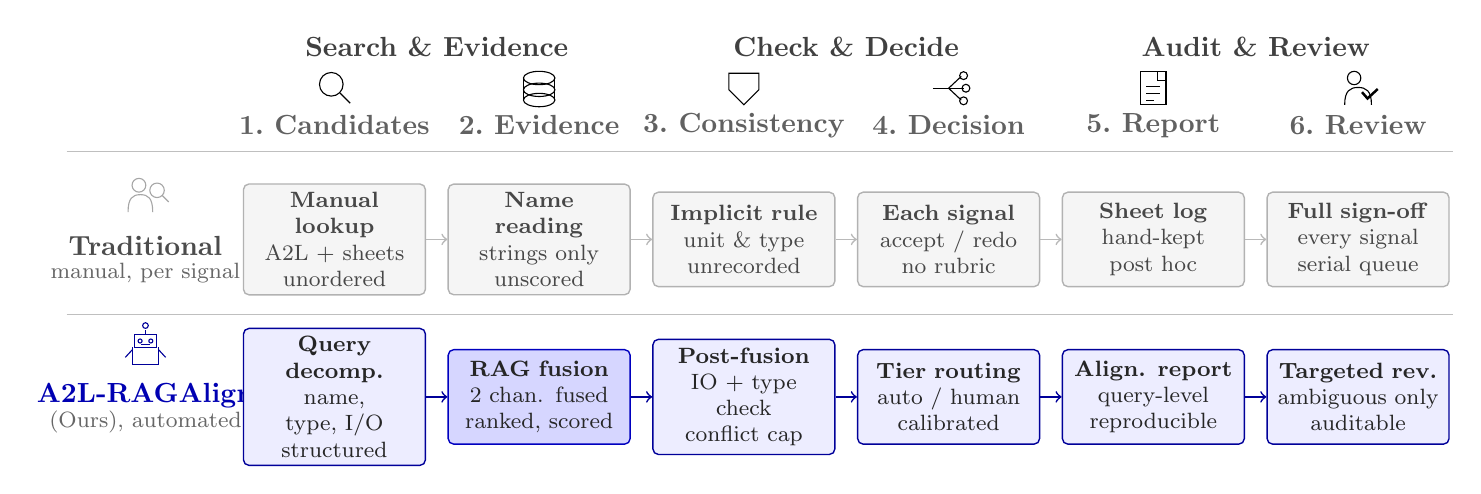
\begin{tikzpicture}[
    font=\footnotesize,
    every node/.style={align=center},
    colhead/.style={font=\bfseries, text=black!62},
    grouplbl/.style={font=\bfseries, text=black!75, fill=white,
                     inner xsep=4pt},
    rowname/.style={font=\bfseries},
    rowsub/.style={text=black!60},
    cell/.style={font=\footnotesize, text width=2.10cm, inner sep=3pt,
               minimum height=1.20cm, line width=0.5pt, rounded corners=2pt},
    man/.style={cell, draw=gray!60, fill=gray!8, text=black!72},
    rag/.style={cell, draw=blue!60!black, fill=blue!7, text=black!85},
    core/.style={rag, draw=blue!75!black, fill=blue!16},
    flowm/.style={->, line width=0.6pt, draw=gray!55},
    flowr/.style={->, line width=0.6pt, draw=blue!60!black},
    rule/.style={line width=0.4pt, draw=black!25},
    grouprule/.style={line width=0.5pt, draw=black!45},
    % ---- stage icons (line art, origin = icon centre) --------------------
    pics/search/.style={code={
        \draw (-0.04,0.05) circle (0.15);
        \draw (0.07,-0.06) -- (0.20,-0.19);}},
    pics/database/.style={code={
        \draw (0,0.13) ellipse (0.20 and 0.085);
        \draw (-0.20,0.13) -- (-0.20,-0.14);
        \draw (0.20,0.13) -- (0.20,-0.14);
        \draw (0,-0.02) ellipse (0.20 and 0.085);
        \draw (0,-0.15) ellipse (0.20 and 0.085);}},
    pics/shield/.style={code={
        \draw (-0.19,0.19) -- (0.19,0.19) -- (0.19,-0.02)
              -- (0,-0.21) -- (-0.19,-0.02) -- cycle;}},
    pics/route/.style={code={
        \draw (-0.20,0.0) -- (0.0,0.0);
        \draw (0.0,0.0) -- (0.16,0.15);
        \draw (0.0,0.0) -- (0.20,0.0);
        \draw (0.0,0.0) -- (0.16,-0.15);
        \draw (0.19,0.16) circle (0.05);
        \draw (0.22,0.0) circle (0.05);
        \draw (0.19,-0.16) circle (0.05);}},
    pics/report/.style={code={
        \draw (-0.16,-0.21) rectangle (0.16,0.21);
        \draw (0.05,0.21) -- (0.05,0.10) -- (0.16,0.10);
        \draw (-0.09,0.02) -- (0.09,0.02);
        \draw (-0.09,-0.07) -- (0.09,-0.07);
        \draw (-0.09,-0.16) -- (0.01,-0.16);}},
    pics/expert/.style={code={
        \draw (-0.05,0.13) circle (0.085);
        \draw (-0.17,-0.21) .. controls (-0.17,-0.03) and (-0.10,0.01)
              .. (0.0,0.01) .. controls (0.10,0.01) and (0.17,-0.03)
              .. (0.17,-0.21);
        \draw[line width=0.9pt] (0.05,-0.05) -- (0.12,-0.13) -- (0.25,-0.01);}},
    pics/person/.style={code={
        \begin{scope}[scale=0.92]
            \draw (-0.09,0.15) circle (0.095);
            \draw (-0.24,-0.22) .. controls (-0.24,-0.03) and (-0.18,0.02) .. (-0.07,0.02)
                  .. controls (0.04,0.02) and (0.10,-0.03) .. (0.10,-0.22);
            \draw (0.16,0.08) circle (0.10);
            \draw (0.23,0.01) -- (0.32,-0.08);
        \end{scope}}},
    pics/robot/.style={code={
        % yshift aligns the visual centre of the robot with the
        % visual centre of the person icon in the row above
        \begin{scope}[scale=0.80, yshift=-0.065cm]
            \draw (0,0.24) -- (0,0.32);
            \draw (0,0.385) circle (0.045);
            \draw (-0.17,0.24) rectangle (0.17,0.04);
            \draw (-0.085,0.14) circle (0.032);
            \draw (0.085,0.14) circle (0.032);
            \draw (-0.07,0.08) -- (0.07,0.08);
            \draw (-0.21,0.04) -- (-0.21,-0.24) -- (0.21,-0.24) -- (0.21,0.04);
            \draw (-0.21,0.0) -- (-0.32,-0.12);
            \draw (0.21,0.0) -- (0.32,-0.12);
        \end{scope}}},
]
% ---------------------------- phase groups ---------------------------------
\draw[grouprule] (3.6,3.45) -- (6.2,3.45);
\draw[grouprule] (3.6,3.45) -- (3.6,3.28);
\draw[grouprule] (6.2,3.45) -- (6.2,3.28);
\node[grouplbl] at (4.9,3.45) {Search \& Evidence};

\draw[grouprule] (8.8,3.45) -- (11.4,3.45);
\draw[grouprule] (8.8,3.45) -- (8.8,3.28);
\draw[grouprule] (11.4,3.45) -- (11.4,3.28);
\node[grouplbl] at (10.1,3.45) {Check \& Decide};

\draw[grouprule] (14.0,3.45) -- (16.6,3.45);
\draw[grouprule] (14.0,3.45) -- (14.0,3.28);
\draw[grouprule] (16.6,3.45) -- (16.6,3.28);
\node[grouplbl] at (15.3,3.45) {Audit \& Review};
% ---------------------------- column headers ------------------------------
\foreach \x/\ic/\t in {3.6/search/{1.\ Candidates},
                       6.2/database/{2.\ Evidence},
                       8.8/shield/{3.\ Consistency},
                       11.4/route/{4.\ Decision},
                       14.0/report/{5.\ Report},
                       16.6/expert/{6.\ Review}} {
    \pic at (\x,2.92) {\ic};
    \node[colhead] at (\x,2.45) {\t};
}
\draw[rule] (0.2,2.12) -- (17.8,2.12);
% ======================= row A: traditional workflow ======================
\begin{scope}[draw=gray!70]
    \pic at (1.2,1.55) {person};
\end{scope}
\node[rowname, text=black!70] at (1.2,0.92) {Traditional};
\node[rowsub] at (1.2,0.58) {manual, per signal};
\node[man] (a1) at (3.6,1.0)
    {\textbf{Manual lookup}\\A2L + sheets\\unordered};
\node[man] (a2) at (6.2,1.0)
    {\textbf{Name reading}\\strings only\\unscored};
\node[man] (a3) at (8.8,1.0)
    {\textbf{Implicit rule}\\unit \& type\\unrecorded};
\node[man] (a4) at (11.4,1.0)
    {\textbf{Each signal}\\accept / redo\\no rubric};
\node[man] (a5) at (14.0,1.0)
    {\textbf{Sheet log}\\hand-kept\\post hoc};
\node[man] (a6) at (16.6,1.0)
    {\textbf{Full sign-off}\\every signal\\serial queue};
\draw[flowm] (a1) -- (a2);
\draw[flowm] (a2) -- (a3);
\draw[flowm] (a3) -- (a4);
\draw[flowm] (a4) -- (a5);
\draw[flowm] (a5) -- (a6);
\draw[rule] (0.2,0.05) -- (17.8,0.05);
% ===================== row B: A2L-RAGAlign (ours) ========================
\begin{scope}[draw=blue!60!black]
    \pic at (1.2,-0.35) {robot};
\end{scope}
\node[rowname, text=blue!70!black] at (1.2,-0.98) {A2L-RAGAlign};
\node[rowsub] at (1.2,-1.32) {(Ours), automated};
\node[rag] (b1) at (3.6,-1.0)
    {\textbf{Query decomp.}\\name, type, I/O\\structured};
\node[core] (b2) at (6.2,-1.0)
    {\textbf{RAG fusion}\\2 chan. fused\\ranked, scored};
\node[rag] (b3) at (8.8,-1.0)
    {\textbf{Post-fusion}\\IO + type check\\conflict cap};
\node[rag] (b4) at (11.4,-1.0)
    {\textbf{Tier routing}\\auto / human\\calibrated};
\node[rag] (b5) at (14.0,-1.0)
    {\textbf{Align. report}\\query-level\\reproducible};
\node[rag] (b6) at (16.6,-1.0)
    {\textbf{Targeted rev.}\\ambiguous only\\auditable};
\draw[flowr] (b1) -- (b2);
\draw[flowr] (b2) -- (b3);
\draw[flowr] (b3) -- (b4);
\draw[flowr] (b4) -- (b5);
\draw[flowr] (b5) -- (b6);
\end{tikzpicture}

%
% ASCII-only on purpose: the paper is built with pdfLaTeX (no CJK support).
%
% Structure: three phase groups (candidate & evidence / validation & decision
% / traceability & review) over six stage columns, one row per workflow.
% Every cell follows the same three-line schema
%
%     <action> / <mechanism> / <outcome property>
%
% so that the two rows are directly comparable column by column, and the
% difference between them reads as "who executes which stage, with what
% machinery, and what is recorded".  All icons are drawn with plain TikZ
% paths: the figure needs no external image files and stays pure vector in
% the typeset PDF.
%
% Cell lines are kept at or below 14 characters so that no cell wraps and
% both rows keep one common baseline grid.
% ---------------------------------------------------------------------------
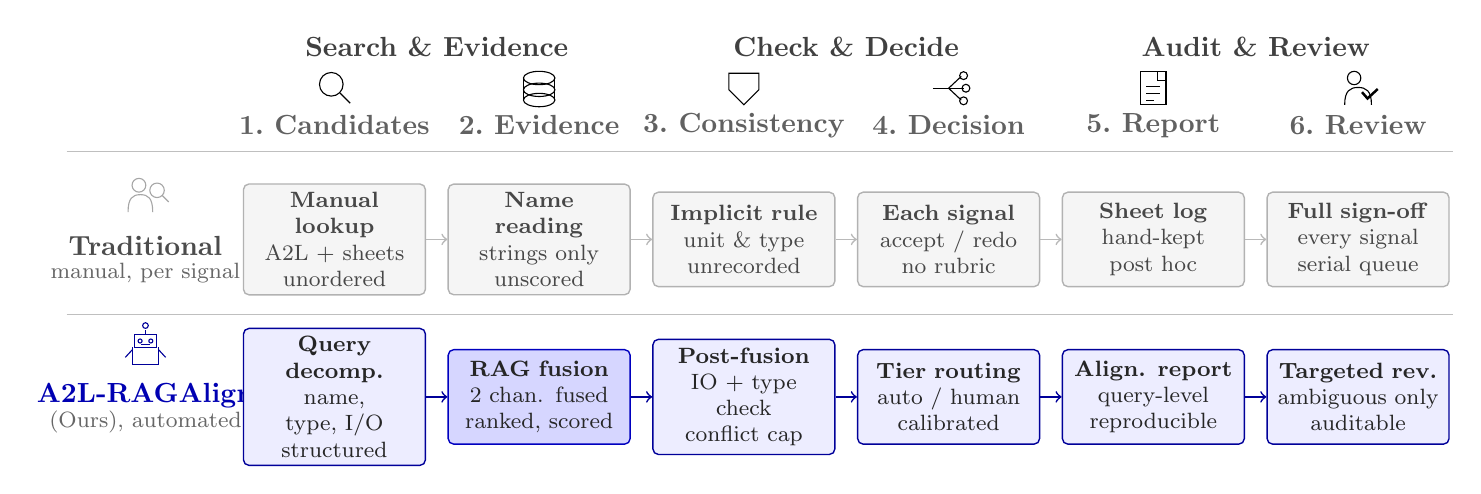
\begin{tikzpicture}[
    font=\footnotesize,
    every node/.style={align=center},
    colhead/.style={font=\bfseries, text=black!62},
    grouplbl/.style={font=\bfseries, text=black!75, fill=white,
                     inner xsep=4pt},
    rowname/.style={font=\bfseries},
    rowsub/.style={text=black!60},
    cell/.style={font=\footnotesize, text width=2.10cm, inner sep=3pt,
               minimum height=1.20cm, line width=0.5pt, rounded corners=2pt},
    man/.style={cell, draw=gray!60, fill=gray!8, text=black!72},
    rag/.style={cell, draw=blue!60!black, fill=blue!7, text=black!85},
    core/.style={rag, draw=blue!75!black, fill=blue!16},
    flowm/.style={->, line width=0.6pt, draw=gray!55},
    flowr/.style={->, line width=0.6pt, draw=blue!60!black},
    rule/.style={line width=0.4pt, draw=black!25},
    grouprule/.style={line width=0.5pt, draw=black!45},
    % ---- stage icons (line art, origin = icon centre) --------------------
    pics/search/.style={code={
        \draw (-0.04,0.05) circle (0.15);
        \draw (0.07,-0.06) -- (0.20,-0.19);}},
    pics/database/.style={code={
        \draw (0,0.13) ellipse (0.20 and 0.085);
        \draw (-0.20,0.13) -- (-0.20,-0.14);
        \draw (0.20,0.13) -- (0.20,-0.14);
        \draw (0,-0.02) ellipse (0.20 and 0.085);
        \draw (0,-0.15) ellipse (0.20 and 0.085);}},
    pics/shield/.style={code={
        \draw (-0.19,0.19) -- (0.19,0.19) -- (0.19,-0.02)
              -- (0,-0.21) -- (-0.19,-0.02) -- cycle;}},
    pics/route/.style={code={
        \draw (-0.20,0.0) -- (0.0,0.0);
        \draw (0.0,0.0) -- (0.16,0.15);
        \draw (0.0,0.0) -- (0.20,0.0);
        \draw (0.0,0.0) -- (0.16,-0.15);
        \draw (0.19,0.16) circle (0.05);
        \draw (0.22,0.0) circle (0.05);
        \draw (0.19,-0.16) circle (0.05);}},
    pics/report/.style={code={
        \draw (-0.16,-0.21) rectangle (0.16,0.21);
        \draw (0.05,0.21) -- (0.05,0.10) -- (0.16,0.10);
        \draw (-0.09,0.02) -- (0.09,0.02);
        \draw (-0.09,-0.07) -- (0.09,-0.07);
        \draw (-0.09,-0.16) -- (0.01,-0.16);}},
    pics/expert/.style={code={
        \draw (-0.05,0.13) circle (0.085);
        \draw (-0.17,-0.21) .. controls (-0.17,-0.03) and (-0.10,0.01)
              .. (0.0,0.01) .. controls (0.10,0.01) and (0.17,-0.03)
              .. (0.17,-0.21);
        \draw[line width=0.9pt] (0.05,-0.05) -- (0.12,-0.13) -- (0.25,-0.01);}},
    pics/person/.style={code={
        \begin{scope}[scale=0.92]
            \draw (-0.09,0.15) circle (0.095);
            \draw (-0.24,-0.22) .. controls (-0.24,-0.03) and (-0.18,0.02) .. (-0.07,0.02)
                  .. controls (0.04,0.02) and (0.10,-0.03) .. (0.10,-0.22);
            \draw (0.16,0.08) circle (0.10);
            \draw (0.23,0.01) -- (0.32,-0.08);
        \end{scope}}},
    pics/robot/.style={code={
        % yshift aligns the visual centre of the robot with the
        % visual centre of the person icon in the row above
        \begin{scope}[scale=0.80, yshift=-0.065cm]
            \draw (0,0.24) -- (0,0.32);
            \draw (0,0.385) circle (0.045);
            \draw (-0.17,0.24) rectangle (0.17,0.04);
            \draw (-0.085,0.14) circle (0.032);
            \draw (0.085,0.14) circle (0.032);
            \draw (-0.07,0.08) -- (0.07,0.08);
            \draw (-0.21,0.04) -- (-0.21,-0.24) -- (0.21,-0.24) -- (0.21,0.04);
            \draw (-0.21,0.0) -- (-0.32,-0.12);
            \draw (0.21,0.0) -- (0.32,-0.12);
        \end{scope}}},
]
% ---------------------------- phase groups ---------------------------------
\draw[grouprule] (3.6,3.45) -- (6.2,3.45);
\draw[grouprule] (3.6,3.45) -- (3.6,3.28);
\draw[grouprule] (6.2,3.45) -- (6.2,3.28);
\node[grouplbl] at (4.9,3.45) {Search \& Evidence};

\draw[grouprule] (8.8,3.45) -- (11.4,3.45);
\draw[grouprule] (8.8,3.45) -- (8.8,3.28);
\draw[grouprule] (11.4,3.45) -- (11.4,3.28);
\node[grouplbl] at (10.1,3.45) {Check \& Decide};

\draw[grouprule] (14.0,3.45) -- (16.6,3.45);
\draw[grouprule] (14.0,3.45) -- (14.0,3.28);
\draw[grouprule] (16.6,3.45) -- (16.6,3.28);
\node[grouplbl] at (15.3,3.45) {Audit \& Review};
% ---------------------------- column headers ------------------------------
\foreach \x/\ic/\t in {3.6/search/{1.\ Candidates},
                       6.2/database/{2.\ Evidence},
                       8.8/shield/{3.\ Consistency},
                       11.4/route/{4.\ Decision},
                       14.0/report/{5.\ Report},
                       16.6/expert/{6.\ Review}} {
    \pic at (\x,2.92) {\ic};
    \node[colhead] at (\x,2.45) {\t};
}
\draw[rule] (0.2,2.12) -- (17.8,2.12);
% ======================= row A: traditional workflow ======================
\begin{scope}[draw=gray!70]
    \pic at (1.2,1.55) {person};
\end{scope}
\node[rowname, text=black!70] at (1.2,0.92) {Traditional};
\node[rowsub] at (1.2,0.58) {manual, per signal};
\node[man] (a1) at (3.6,1.0)
    {\textbf{Manual lookup}\\A2L + sheets\\unordered};
\node[man] (a2) at (6.2,1.0)
    {\textbf{Name reading}\\strings only\\unscored};
\node[man] (a3) at (8.8,1.0)
    {\textbf{Implicit rule}\\unit \& type\\unrecorded};
\node[man] (a4) at (11.4,1.0)
    {\textbf{Each signal}\\accept / redo\\no rubric};
\node[man] (a5) at (14.0,1.0)
    {\textbf{Sheet log}\\hand-kept\\post hoc};
\node[man] (a6) at (16.6,1.0)
    {\textbf{Full sign-off}\\every signal\\serial queue};
\draw[flowm] (a1) -- (a2);
\draw[flowm] (a2) -- (a3);
\draw[flowm] (a3) -- (a4);
\draw[flowm] (a4) -- (a5);
\draw[flowm] (a5) -- (a6);
\draw[rule] (0.2,0.05) -- (17.8,0.05);
% ===================== row B: A2L-RAGAlign (ours) ========================
\begin{scope}[draw=blue!60!black]
    \pic at (1.2,-0.35) {robot};
\end{scope}
\node[rowname, text=blue!70!black] at (1.2,-0.98) {A2L-RAGAlign};
\node[rowsub] at (1.2,-1.32) {(Ours), automated};
\node[rag] (b1) at (3.6,-1.0)
    {\textbf{Query decomp.}\\name, type, I/O\\structured};
\node[core] (b2) at (6.2,-1.0)
    {\textbf{RAG fusion}\\2 chan. fused\\ranked, scored};
\node[rag] (b3) at (8.8,-1.0)
    {\textbf{Post-fusion}\\IO + type check\\conflict cap};
\node[rag] (b4) at (11.4,-1.0)
    {\textbf{Tier routing}\\auto / human\\calibrated};
\node[rag] (b5) at (14.0,-1.0)
    {\textbf{Align. report}\\query-level\\reproducible};
\node[rag] (b6) at (16.6,-1.0)
    {\textbf{Targeted rev.}\\ambiguous only\\auditable};
\draw[flowr] (b1) -- (b2);
\draw[flowr] (b2) -- (b3);
\draw[flowr] (b3) -- (b4);
\draw[flowr] (b4) -- (b5);
\draw[flowr] (b5) -- (b6);
\end{tikzpicture}
